% In this section, the layer is described in some detail in terms of its specific subsystems. Describe each of the layers and its subsystems in a separate chapter/major subsection of this document. The content of each subsystem description should be similar. Include in this section any special considerations and/or trade-offs considered for the approach you have chosen.

The pathfinding subsystem manages the components or modules within a larger pathfinding system that handles specific aspects of the 

\subsection{Grid Management Subsystem}
The grid management subsystem allows the display of the LiDAR range as a grid of cells and allows them to be marked as either traversable or non-traversable, as needed.

% This section should be a general description of a particular subsystem for the given layer. For most subsystems, an extract of the architectural block diagram with data flows is useful. This should consist of the subsystem being described and those subsystems with which it communicates.


%%%%%%%%%%%%%%%%%%%%%%%%%%%%%%%%%%%%%%%%%%%%%%%%%%%%%%%%%%%%%%%%%%%%%%%%%%%%
%   Change the graphic here. Put your image in the 'images' folder
%   and update the name from 'images/test_image' to your image name
\begin{figure}[h!]
	\centering
 	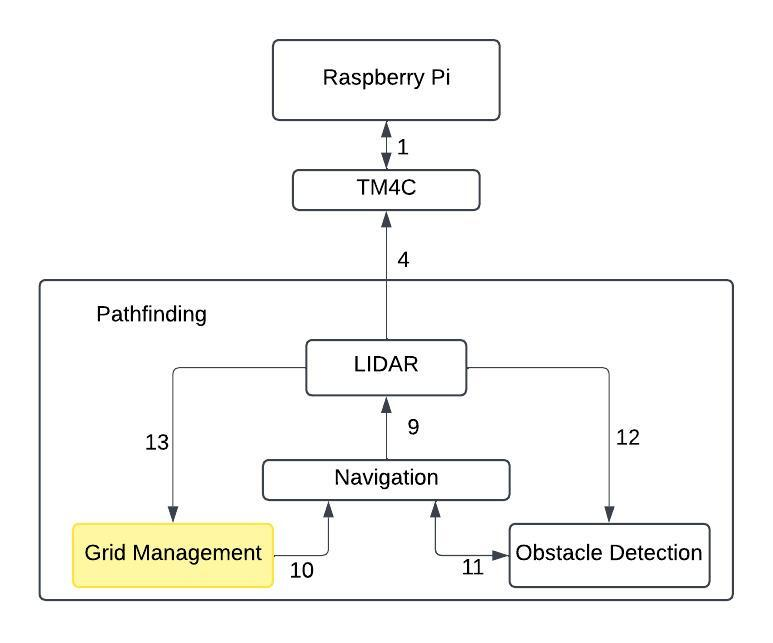
\includegraphics[width=0.80\textwidth]{images/pathfinding_images/GridManagement.jpeg}
 \caption{Pathfinding Subsystem - Grid Management} % Be sure to change the caption.
\end{figure}

\subsubsection{Assumptions}
% Any assumptions made in the definition of the subsystem should be listed and described. Pay particular attention to assumptions concerning interfaces and interactions with other layers.

Grid management allows for the environment within the LiDAR range to be modeled to a graph or grid. All cells within in the grid shall either be marked as traversable or non-traversable depending on if an obstacle is within the cell. The grid will dynamically update itself once it nears the outer area of the grid or when new obstacles are introduced.
\subsubsection{Responsibilities}
% Each of the responsibilities/features/functions/services of the subsystem as identified in the architectural summary must be expanded to more detailed responsibilities. These responsibilities form the basis for the identification of the finer-grained responsibilities of the layer's internal subsystems. Clearly describe what each subsystem does.

The pathfinding algorithm creates a grid representing the environment with the LiDAR Range. The grid will contain nodes that contain properties such as: 
\begin{itemize}
  \item Traverability (true/false).
  \item Coordinates in world space.
\end{itemize}
The pathfinding algorithm will also covert world space coordinates to cells, and allow to update nodes during a terrain change.
\subsubsection{Subsystem Interfaces}
% Each of the inputs and outputs for the subsystem are defined here. Create a table with an entry for each labelled interface that connects to this subsystem. For each entry, describe any incoming and outgoing data elements will pass through this interface.

\begin {table}[H]
\caption {Pathfinding Subsystem - Grid Management} 
\begin{center}
    \begin{tabular}{ | p{1.2cm} | p{6cm} | p{3cm} | p{3cm} |}
    \hline
    ID & Description & Inputs & Outputs \\ \hline
    \#10/13 & Data that will create a cells within a grid & \pbox{3cm}{World Coordinates} & \pbox{3cm}{Node Data}  \\ \hline

    \end{tabular}
\end{center}
\end{table}

\subsection{Obstacle Detection Subsystems}
The obstacle detection subsystem is designed to process feedback from the LiDAR, identifying objects within its range and marking them as impassable when necessary.
%%%%%%%%%%%%%%%%%%%%%%%%%%%%%%%%%%%%%%%%%%%%%%%%%%%%%%%%%%%%%%%%%%%%%%%%%%%%
%   Change the graphic here. Put your image in the 'images' folder
%   and update the name from 'images/test_image' to your image name
\begin{figure}[h!]
	\centering
 	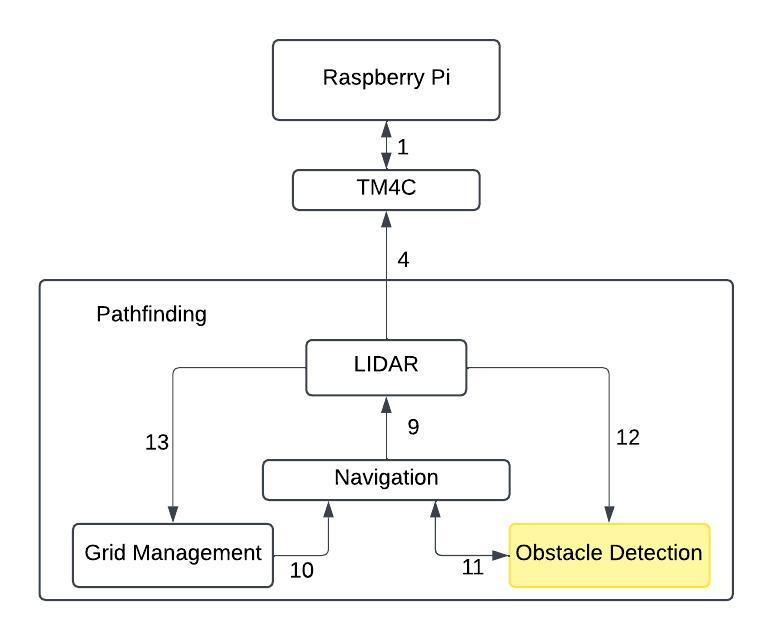
\includegraphics[width=0.60\textwidth]{images/pathfinding_images/ObstacleDetection.jpeg}
 \caption{Pathfinding Subsystem - Obstacle Detection} % Be sure to change the caption.
\end{figure}

\subsubsection{Assumptions}
% Any assumptions made in the definition of the subsystem should be listed and described. Pay particular attention to assumptions concerning interfaces and interactions with other layers.
The rover will be able to register static and dynamic obstacles and be detected with LiDAR.
\subsubsection{Responsibilities}
% Each of the responsibilities/features/functions/services of the subsystem as identified in the architectural summary must be expanded to more detailed responsibilities. These responsibilities form the basis for the identification of the finer-grained responsibilities of the layer's internal subsystems. Clearly describe what each subsystem does.

The rover will be able to detect obstacles and update the graph representation Subsystem by marking a cell as untraversable. The obstacle detection subsystem should also be able to be integrated with LiDAR and other sensors. If the close-range sensors get triggered the rover should halt movement and retreat a set distance before reactivating its pathfinding.

\subsubsection{Subsystem Interfaces}
% Each of the inputs and outputs for the subsystem are defined here. Create a table with an entry for each labelled interface that connects to this subsystem. For each entry, describe any incoming and outgoing data elements will pass through this interface.

\begin {table}[H]
\caption {Pathfinding Subsystem - Obstacle Detection} 
\begin{center}
    \begin{tabular}{ | p{1.2cm} | p{6cm} | p{3cm} | p{3cm} |}
    \hline
    ID & Description & Inputs & Outputs \\ \hline
    \#11/12 & Algorithm will send a signal to the Navigation sending marked obstacles& \pbox{3cm}{Input from LiDAR} & \pbox{3cm}{ Obstacle Update Signals}  \\ \hline

    \end{tabular}
\end{center}
\end{table}

\subsection{Navigation Subsystems}
The pathfinding subsystem is designed to give the Roam\_Bot the ability to traverse the terrain and reach the desired terrain.
%%%%%%%%%%%%%%%%%%%%%%%%%%%%%%%%%%%%%%%%%%%%%%%%%%%%%%%%%%%%%%%%%%%%%%%%%%%%
%   Change the graphic here. Put your image in the 'images' folder
%   and update the name from 'images/test_image' to your image name
\begin{figure}[h!]
	\centering
 	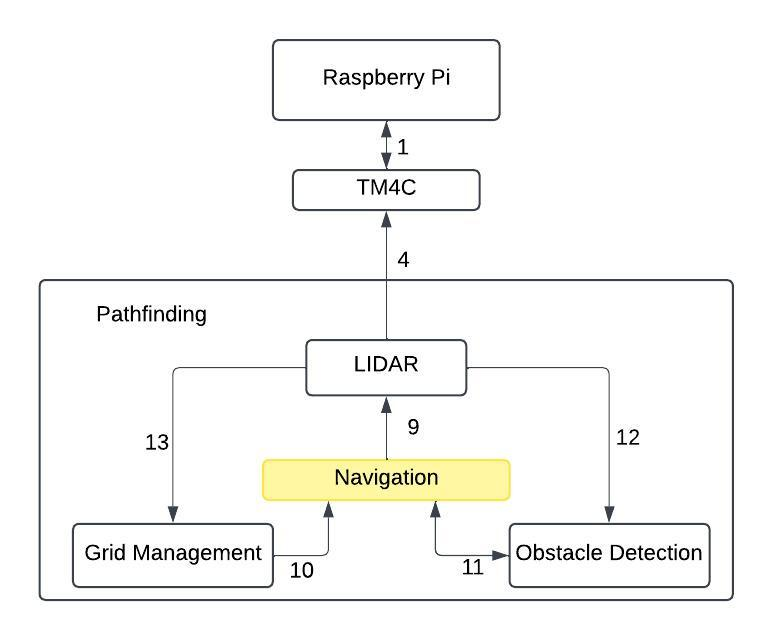
\includegraphics[width=0.60\textwidth]{images/pathfinding_images/Navigation.jpeg}
 \caption{Pathfinding Subsystem - Navigation} % Be sure to change the caption.
\end{figure}

\subsubsection{Assumptions}
% Any assumptions made in the definition of the subsystem should be listed and described. Pay particular attention to assumptions concerning interfaces and interactions with other layers.

The pathfinding algorithm requires that the graph is already constructed, and LiDAR is active.
\subsubsection{Responsibilities}
% Each of the responsibilities/features/functions/services of the subsystem as identified in the architectural summary must be expanded to more detailed responsibilities. These responsibilities form the basis for the identification of the finer-grained responsibilities of the layer's internal subsystems. Clearly describe what each subsystem does.

The pathfinding algorithm calculates either the optimal or heuristic-based path from a start to end node. The pathfinding algorithms should also allow for multiple algorithms such as A*, Djiksta's, Breadth-First-Search, etc. While also handling-handling static and dynamic obstacles.
\subsubsection{Subsystem Interfaces}
% Each of the inputs and outputs for the subsystem are defined here. Create a table with an entry for each labelled interface that connects to this subsystem. For each entry, describe any incoming and outgoing data elements will pass through this interface.

\begin {table}[H]
\caption {Pathfinding Subsystem - Navigation} 
\begin{center}
    \begin{tabular}{ | p{1.8cm} | p{6cm} | p{3cm} | p{3cm} |}
    \hline
    ID & Description & Inputs & Outputs \\ \hline
    \#9/10/11 & Algorithm will feed pathfinding to LiDAR Range& \pbox{3cm}{Navigation} & \pbox{3cm}{Data to TM4C (Microcontroller)}  \\ \hline

    \end{tabular}
\end{center}
\end{table}

\subsection{LiDAR Subsystems}
The LiDAR subsystem is designed to give the Roam\_Bot the ability to see the desired terrain.
%%%%%%%%%%%%%%%%%%%%%%%%%%%%%%%%%%%%%%%%%%%%%%%%%%%%%%%%%%%%%%%%%%%%%%%%%%%%
%   Change the graphic here. Put your image in the 'images' folder
%   and update the name from 'images/test_image' to your image name
\begin{figure}[h!]
	\centering
 	\includegraphics[width=0.60\textwidth]{images/pathfinding_images/LiDAR.jpeg}
 \caption{Pathfinding Subsystem - LiDAR} % Be sure to change the caption.
\end{figure}

\subsubsection{Assumptions}
% Any assumptions made in the definition of the subsystem should be listed and described. Pay particular attention to assumptions concerning interfaces and interactions with other layers.

The LiDAR subsystem requires that the Roam\_Bot be turned on.
\subsubsection{Responsibilities}
% Each of the responsibilities/features/functions/services of the subsystem as identified in the architectural summary must be expanded to more detailed responsibilities. These responsibilities form the basis for the identification of the finer-grained responsibilities of the layer's internal subsystems. Clearly describe what each subsystem does.

The LiDAR subsystem takes the input given by its senses and sends all relavant information to the Grid Management, and Obstacle Detection subsystems as well as the TM4C system.

\subsubsection{Subsystem Interfaces}


% Each of the inputs and outputs for the subsystem are defined here. Create a table with an entry for each labelled interface that connects to this subsystem. For each entry, describe any incoming and outgoing data elements will pass through this interface.

\begin {table}[H]
\caption {Pathfinding Subsystem - LiDAR} 
\begin{center}
    \begin{tabular}{ | p{1cm} | p{6cm} | p{3cm} | p{3cm} |}
    \hline
    ID & Description & Inputs & Outputs \\ \hline
    \#13 &  The LiDAR subsystem will transmit video data to the Grid Management subsystem, which will process the input, convert it into a structured grid, and divide it into individual cells for further analysis.
    & \pbox{3cm}{Navigation} & \pbox{3cm}{Data to TM4C (Microcontroller)}  \\ \hline
    \#12 & 
    The LiDAR subsystem will transmit video data to the Obstacle Detection subsystem, which will analyze the input to identify and classify areas as either obstacles or traversable terrain.
    & \pbox{3cm}{N/A} & \pbox{3cm}{Data to TM4C (Microcontroller)}  \\ \hline
    \#4 & LiDAR will feed accumlated infromation to TM4C (microcontroller)& \pbox{3cm}{Data from Navigation} & \pbox{3cm}{Data to TM4C (Microcontroller)}  \\ \hline
    \end{tabular}
\end{center}
\end{table}
